\chapter{ทดสอบ}
\label{Ch:TEST}

\section{ทดสอบ 1}
โชกี้ บทที่\ref{Ch:TEST} {\boldfont ตัวหนา} {\italicfont ตัวเอียง} \underline{วิทยาศาสตร์} \\นางฟ้า IT

Hello Dear

\subsection{ทดสอบย่อย 1}

\section{ทดสอบ 2}
\begin{itemize}
    \item first item
    จิตรกัณฐ์ ดำรงตระกูลวัฒน์
    \item second item
    \item third item
\end{itemize}

\begin{enumerate}
    \item first item
    \item second item
    \item third item
\end{enumerate}

\begin{table}[]
    \centering
    \begin{tabular}{c|c}
         &  \\
         & 
    \end{tabular}
    \caption{Caption}
    \label{tab:placeholder}
\end{table}

\cite{parker2020}

ตัวอย่างการเพิ่มตารางและการอ้างอิงไปยังตาราง \ref{table:example_table}.

\begin{table}[h]
\centering
\begin{tabular}{|c c c|}
\hline
คอลัมน์1 & คอลัมน์2 & คอลัมน์3 \\ 
\hline
A & xx & xx \\ 
\hline
B & yy & yy \\ 
\hline
C & xx & xx  \\
%\hline
E & ZZ & ZZ \\
\hline
\end{tabular}
\captionsetup{justification=centering, name=ตาราง}
\caption{คำบรรยายตาราง}
\label{table:example_table}
\end{table}

ตัวอย่างการอ้างอิงไปยังบทความในเอกสารอ้างอิง \cite{parker2020}. 

วิธีการเพิ่มรูปภาพและอ้างอิงไปยังรูปภาพ \ref{fig:example_figure}

\begin{figure}[h]
    \centering
    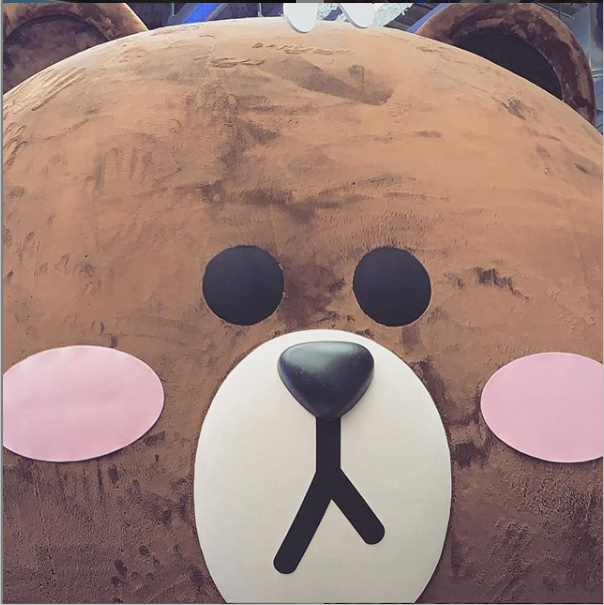
\includegraphics[scale = 0.3]{figures/chap2/Sample101.PNG}
    \captionsetup{name = รูป}
    \caption{คำอธิบายรูปภาพ}
    \label{fig:example_figure}
\end{figure}

วิธีการเพิ่ม{\boldfont สมการ} และ{\italicfont อ้างอิง}ไปยังสมการ \ref{eq:example_equation}.

\begin{equation} 
y = \sqrt{x^2+1}
\label{eq:example_equation}
\end{equation}

\begin{equation}
    x=\frac{a}{b}
    X=\sum_{i=1}^{n} x_1
\end{equation}

\begin{itemize}
    \item AST Parser
    \item ชุดกฎ Green Code Smell
        \begin{itemize}
            \item Long Loop Without Break
            \item Repeated Object Creation
            \item Unnecessary I/O Operations
            \item Inefficient Collection Usage
        \end{itemize}
    \item Metric \& Analysis Module
    \item Reporting Module
\end{itemize}